%%=============================================================================
%% Methodologie
%%=============================================================================

\chapter{\IfLanguageName{dutch}{Methodologie}{Methodology}}
\label{ch:methodologie}

%% TODO: Hoe ben je te werk gegaan? Verdeel je onderzoek in grote fasen, en
%% licht in elke fase toe welke stappen je gevolgd hebt. Verantwoord waarom je
%% op deze manier te werk gegaan bent. Je moet kunnen aantonen dat je de best
%% mogelijke manier toegepast hebt om een antwoord te vinden op de
%% onderzoeksvraag.

In dit onderdeel zal de onderzoeksvraag 'Kunnen we een chatbot automatisch laten bijleren op basis van het gedrag van gebruikers?' onderzocht worden. Hierin zal er gekeken worden naar enkele van de meest bekendste frameworks voor chatbots te kunnen trainen. Het is zeer belangrijk dat hierbij de API van deze frameworks toegankelijk zijn en de juiste methoden bevat zodat de input van de gebruiker kan verwerkt worden op de juiste manier.

\section{Mogelijkheden}
\label{sec:Mogelijkheden}

Eerst en vooral was er voorbereiding nodig want er was nog niet echt ervaring op vlak van chatbots. Wat zijn de mogelijkheden van zo een chatbot framework? Hoe worden intents aangemaakt en hoe werken die? Hoe worden entities aangemaakt en hoe voeg je die toe aan een bepaalde intent? Hoe wordt de bot getraind? Hoe wordt er dan effectief omgegaan met de input van de gebruiker waarbij de bot niet goed weet bij welke intent die hoort en hoe koppel je deze dan aan de juiste intent? Wat kun je nog allemaal met zo een framework doen? Hoe gebruik ik de API? Op al deze vragen zocht ik een antwoord.

\subsection{Ontdekken}
\label{Ontdekken}

De keuze van het eerste framework voor de eerste ervaringen op te doen was niet zo moeilijk. Hierbij kwam LUIS.ai al snel naar boven doordat er op het stagebedrijf al gewerkt wordt hiermee en er een voorbeeld ter beschikking was gesteld waarop er kon worden verder gebouwd.

Het trainen van een chatbot via LUIS is zeer gebruiksvriendelijk. Eerst en vooral dient er een nieuwe app te worden aangemaakt. Dit is zeer eenvoudig door de vereiste naam, de taal die er zal gesproken worden tegen de bot en eventueel een beschrijving toe te voegen. Eénmaal de app is gecreërd dienen er Intents aangemaakt te worden. Een voorbeeld van een intent kan zijn "Greeting", hierin vallen dus alle begroetingen. Per intent dien je dan utterances toe te voegen. Utterances zijn voorbeeldzinnen die worden gelinkt met deze gemaakte intent. Door deze voorbeeldzinnen weet LUIS wat een "Greeting" is. Een voorbeeld die zou passen bij een begroeting is "Hi, I'm Ivor". Hoe meer zinnen je toevoegd, liefst allemaal met een verschillende zinsbouw, hoe beter LUIS de input van de gebruikers zal herkennen en aan deze intent zal linken.


\begin{figure}[h!]
	\centering
	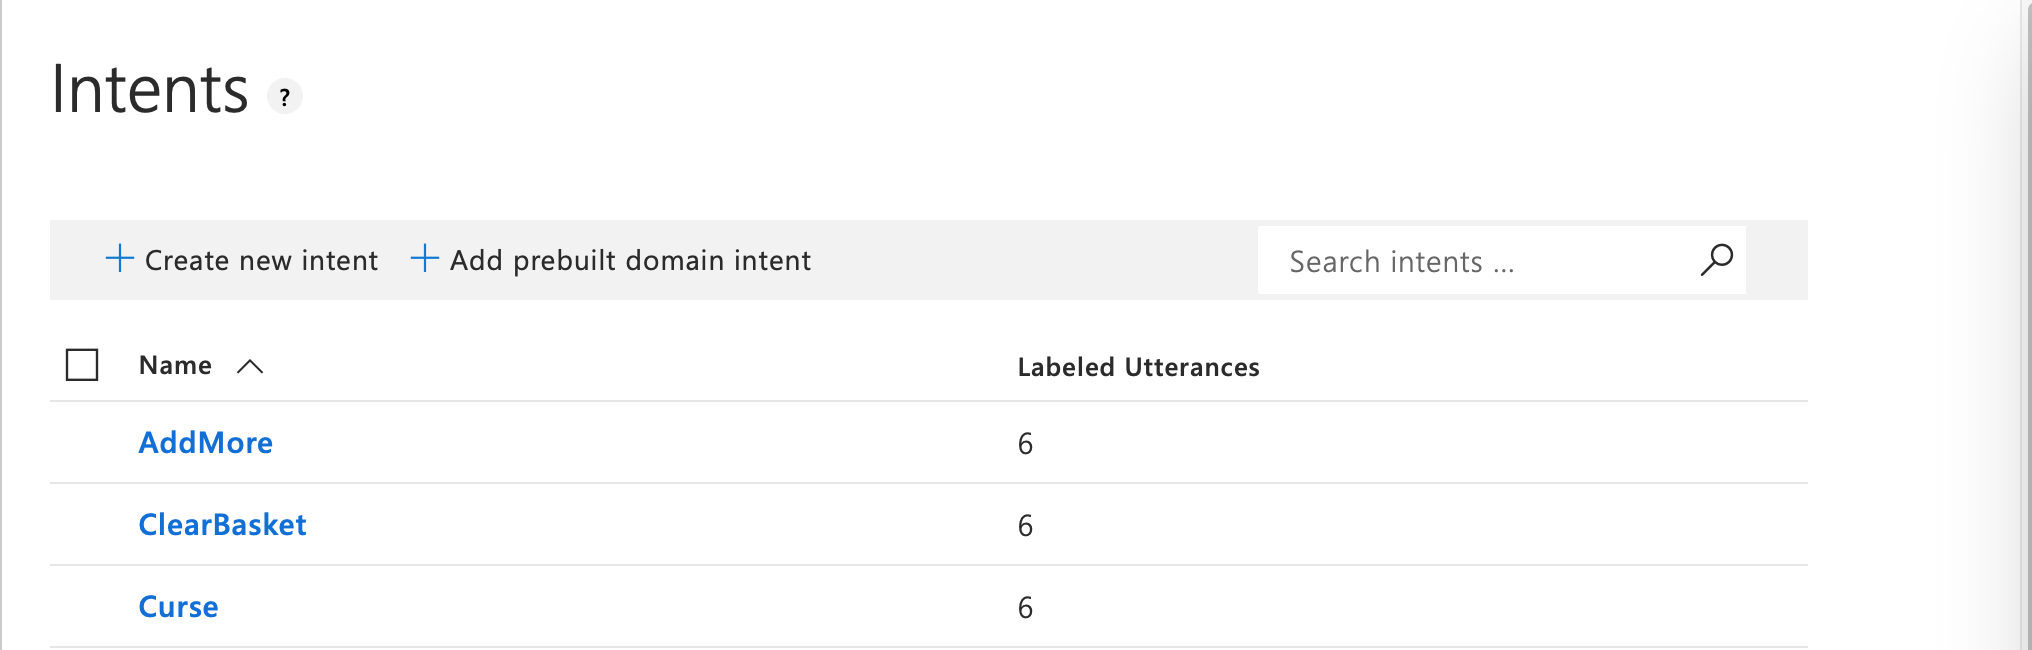
\includegraphics[height=4cm]{img/intents.png}
	\caption{Intent aanmaken Luis.ai}
	\label{fig:intents}
\end{figure}

In de meeste gevallen is een utterance toevoegen niet zomaar eenvoudigweg een zin toevoegen. Meestal zal er in een utterance één of meerdere entities terug te vinden zijn. Bijvoorbeeld in voorgaan voorbeeld bij de intent "Greeting" konden we een utterance toevoegen "Hello, I'm Ivor". In deze utterance is Ivor een entity, namelijk een naam. Het voordeel van deze entities uit de zinnen te halen is dat bijvoorbeeld de chatbot dan al direct weet dat "Ivor" de naam is van de persoon die communiceert met de bot en kan de bot deze persoon aanspreken met zijn naam. Dit maakt het gesprek al persoonlijker.

LUIS heeft zelf al een redelijk aantal ingebouwde entities, zoals nummers, leeftijden, e-mail adressen, ... en kan deze makkelijk zelf al herkennen. Indien er geen ingebouwde entity bestaat kan je zelf een entity maken en deze makkelijk linken aan het juiste woord in een utterance.

\begin{figure}[h!]
	\centering
	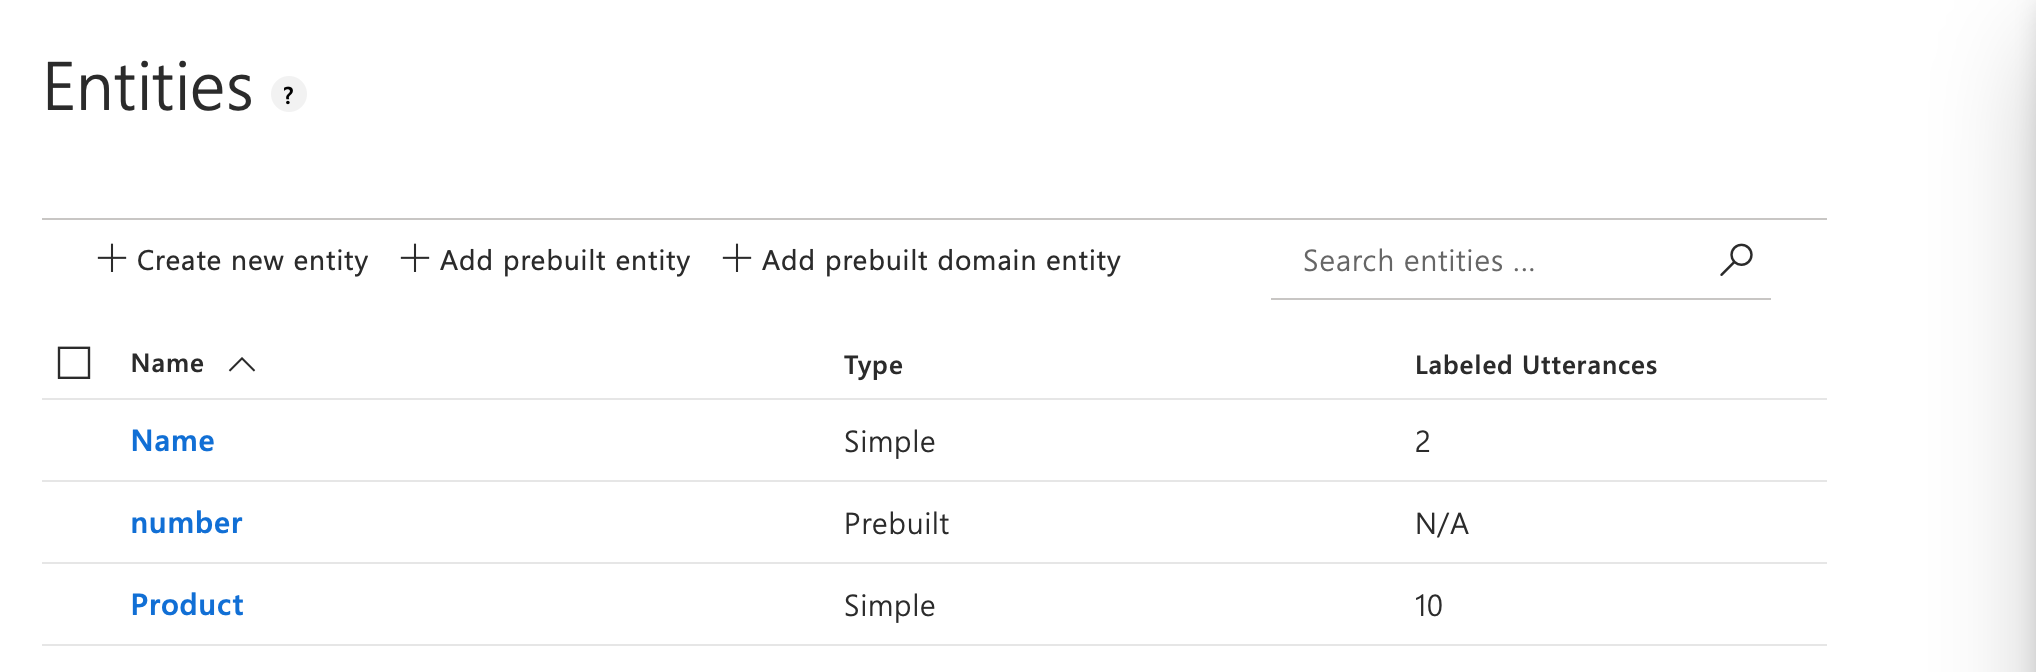
\includegraphics[height=4cm]{img/entity.png}
	\caption{Entities aanmaken Luis.ai}
	\label{fig:entity}
\end{figure}

Eénmaal je enkele intents aangemaakt hebt en bij elke intent enkele utterances hebt toegevoegd (het is aangeraden van er minimum 5 toe te voegen voor een betere accuraatheid) met daarbij eventueel de gepaste entities kan de chatbot als eens gestest worden.

Het enige dat nog moet gebeuren vooraleer er kan getest worden is LUIS trainen. Na het toevoegen van nieuwe intents, entities en utterances dient LUIS opnieuw getraint te worden met de nieuwe data. Na enkele seconden trainen staat alles klaar om getest te worden.

Op de site van LUIS zelf kan er gepraat worden met de chatbot via een simpele interface. Hierin kan er simpelweg gepraat worden met de bot door utterances in te geven. Als voorbeeld kan er weer gebruik worden gemaakt van de utterance: "Hi, I'm Ivor". Zo kun je zien of deze de juiste intent herkent en de entity er juist uithaald met daarbij het percentage van de zekerheid dat LUIS juist is. Bij dit voorbeeld is LUIS er 81 percent zeker van dat deze utterance hoort bij de intent "Greeting" met de entity "Ivor" als "name".

Indien de utterance niet hoort bij de door LUIS geslecteerde intent kan deze handmatig aangepast worden naar de correcte en kan LUIS opnieuw getraind worden zodat dit de volgende keer correct is.

\begin{figure}[h!]
	\centering
	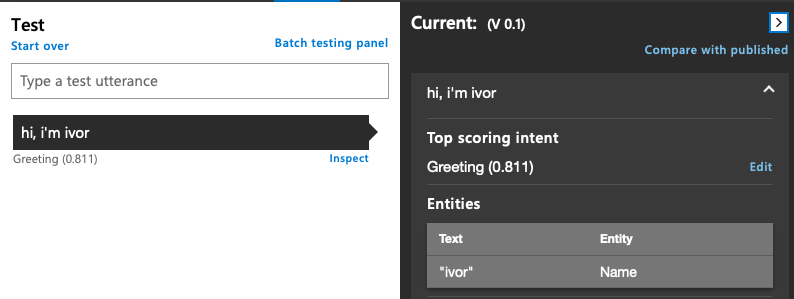
\includegraphics[height=4cm]{img/test.png}
	\caption{Testen van de chatbot Luis.ai}
	\label{fig:test}
\end{figure}

Als alles goed verloopt en bij het testen zijn er niet veel fouten, kan de applicatie geplubliceerd worden. Dit zorgt ervoor dat je vanuit je eigen applicatie de chatbot kan integreren.

Eénmaal deze geïntegreerd is in een eigen applicatie kan er locaal getest worden op wat de chatbot reageert op bepaalde utterances. Dit kan makkelijk getest worden via de "Bot Framework Emulator". Dit is een zeer handig applicatie voor het testen van de bot. Er is een interface zodat het direct lijkt op een echt chatvenster. Hiernaast is er ook een inspector. Hierin komen alle GET en POST boodschappen die worden gestuurd en ontvangen. Zo kan je makkelijk zien als er iets is misgelopen.

\begin{figure}[h!]
	\centering
	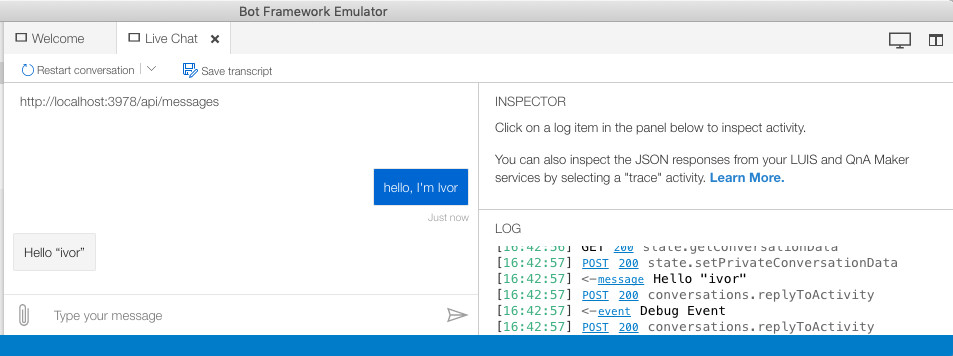
\includegraphics[height=4cm]{img/emulator.png}
	\caption{Bot Framework Emulator}
	\label{fig:emulator}
\end{figure}

Als je LUIS applicatie gepubliceerd is en deze ontvangt input van gebruikers door bijvoorbeeld via de Bot Framework Emulator, analyseert LUIS elk van deze utterances. LUIS probeert die dan te linken aan de juiste intent. LUIS zal nooit 100 percent zeker zijn dat een bepaalde utterance behoort tot één specifieke intent. LUIS zal de utterances die de gebruiker invoert waar hij niet zo zeker van is verzamelen onder "Review endpoint utterances". Onder deze pagina bevinden zich alle utterances waar LUIS minder zeker van is zodat je deze manueel kan linken aan de juiste intent, utterance per utterance. Bij elke utterance geeft LUIS zelf al een schatting bij welke intent elke deze hoort. Afbeelding \ref{fig:review} toont de schattingen van LUIS aan de hand van het percentage dat hij zeker is dat de utterance bij een bepaalde intent hoort. Als deze juist is kan deze toegevoegd worden. 

Indien dit niet juist is, kan er via een dropdown menu de juiste intent geselecteerd worden en deze dan handmatig toevoegen. Bij deze dropdown staan alle intents in volgorde van zekerheid met het percentage erbij. Bij dit voorbeeld "Let's add 3 more" is de gesuggereerde intent van LUIS AddMore met een percentage van 89.2 percent. De tweede suggestie is FintItem met een percentage van 1.8 percent. Door het grote verschil aan percentages wordt er niet getwijfelt dat deze utterance hoort bij de intent "AddMore". De entities van elk van deze utterances worden door LUIS automatisch gedetecteerd. Moest het zijn dat LUIS dat niet gedaan heeft kan je de entities handmatig aanduiden.

\begin{figure}[h!]
	\centering
	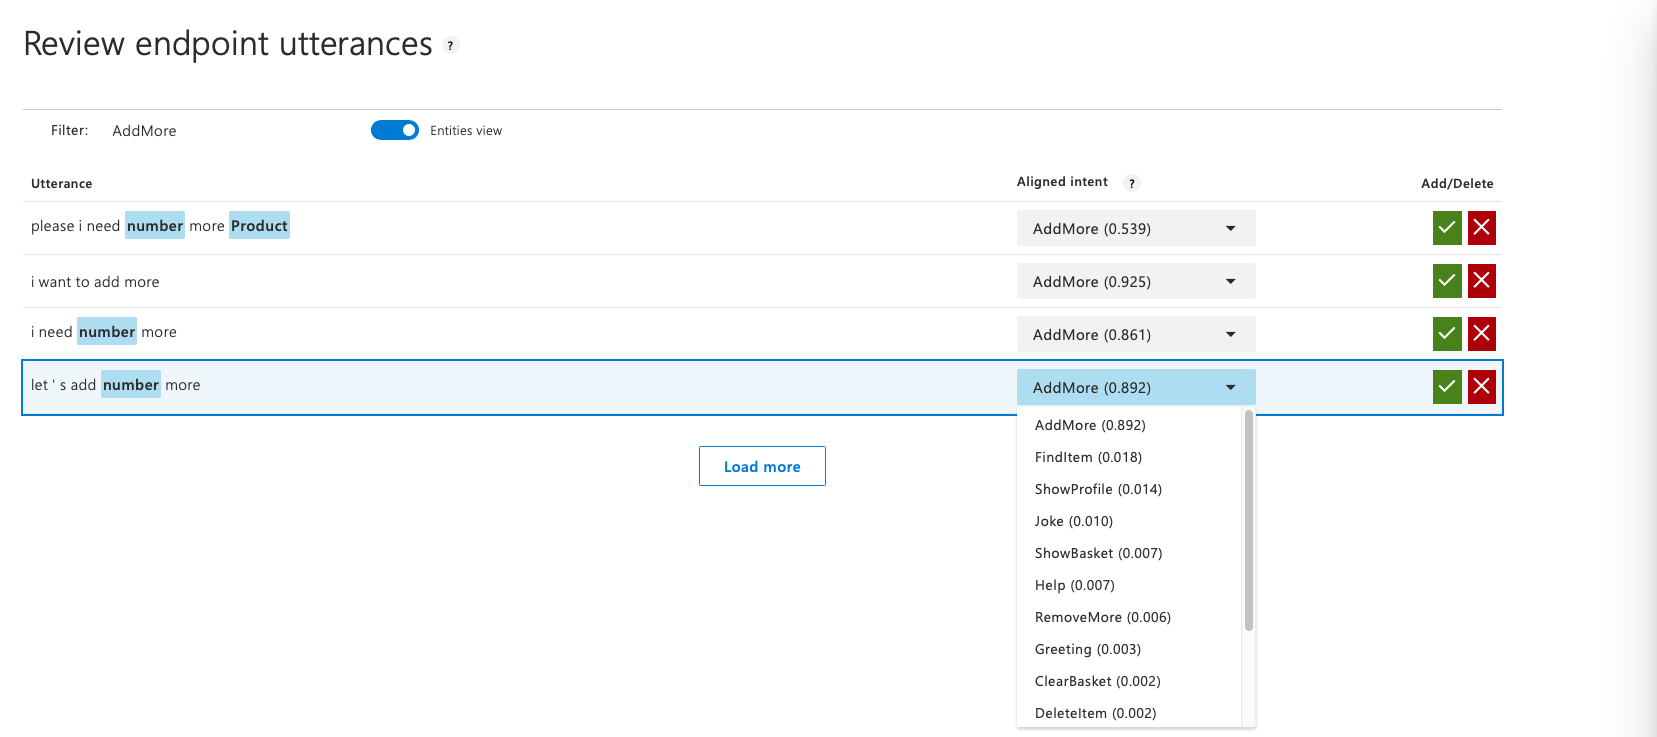
\includegraphics[height=6cm]{img/review.png}
	\caption{Review endpoint utterances Luis.ai}
	\label{fig:review}
\end{figure}

Dit was een zeer goed begin om te begrijpen wat de concepten zijn van een framework voor het ontwikkelen van chatbots. Door het op voorhand bestuderen van één bepaald framework voor het maken van chatbots worden al veel aspecten zeer duidelijk en deze zijn meestal wel hetzelfde voor de andere frameworks ook. Door LUIS al eens te bestuderen is het doel van deze bachelorproef direct veel duidelijk geworden. De review endpoint utterances uit afbeelding \ref{fig:review} dient nu allemaal handmatig te worden goedgekeurd en nagekeken. Zoals er kan gezien worden is het niet nodig om bij elke utterance handmatige controle te steken. Soms is de score van de eerste en de tweede gesuggereerde intent zo groot dat er geen twijfel mogelijk is bij welke intent deze behoort. Bij alle utterances waarbij dit het geval is zou deze handmatige controle achterwege kunnen worden gelaten.

In het volgende deel worden verschillende van de bekendste frameworks voor het maken van bot vergeleken. Hierbij zal gekeken worden of deze een API hebben en of deze toegankelijk genoeg is voor de 'review endpoint utterances' op te halen en deze via een API-call op te halen in een eigen applicatie, deze automatisch te controleren en goedkeuren indien dit kan. Zo zullen uiteindelijk de utterances die nog handmatig zullen moeten gecontroleerd worden veel minder zijn.

\section{Frameworks}
\label{sec:Frameworks}

\subsection{LUIS}
\label{Luis}

Nu dat de basisconcepten van LUIS duidelijk zijn door het vorige hoofdstuk, kan er worden gekeken of LUIS een API heeft en of deze toegankelijk genoeg is voor de onderzoeksvraag te kunnen oplossen. Al snel is duidelijk dat er effectief een API bestaat genaamd 'LUIS Programmatic APIs v2.0'. Hierin is er een grote variatie, van het toevoegen van intents en entities naar het toevoegen van een nieuwe utterance en meer. Voor het ophalen van utterances is er één API-call 'Review labeled examples'. Deze call heeft enkel de utterances weer die al zijn toegevoegd aan een bepaalde intent dus jammer genoeg niet de 'unlabeled examples'. De utterances waarvan LUIS niet exact weet bij welke intent deze hoort, die op de site van LUIS zelf onder 'review endpoint utterances' staan kunnen niet worden opgehaald via een API-call en kunnen dus niet automatisch gecontroleerd worden.

\subsection{Wit.ai}
\label{Wit}

Wit.ai hoort ook bij één van de bekendste frameworks voor het ontwikkelen van chatbots. De grote lijnen van dit framework zijn wat hetzelfde als die van LUIS.

Eerst en vooral moet er een applicatie worden aangemaakt met de naam, de taal waarin de bot zal functioneren en eventueel een omschrijving. Het toevoegen van intents en utterances werkt op een verschillende manier maar komt uiteindelijk op hetzelfde neer. Afbeelding \ref{fig:intentsWit} toont hoe dit in zijn werk gaat. Hier moet je beginnen met het invoeren van een utterance en dan kan deze gelinkt worden met een intent. Hier kunnen we weer het voorbeeld gebruiken van 'Hi, I'm Ivor'.

\begin{figure}[h!]
	\centering
	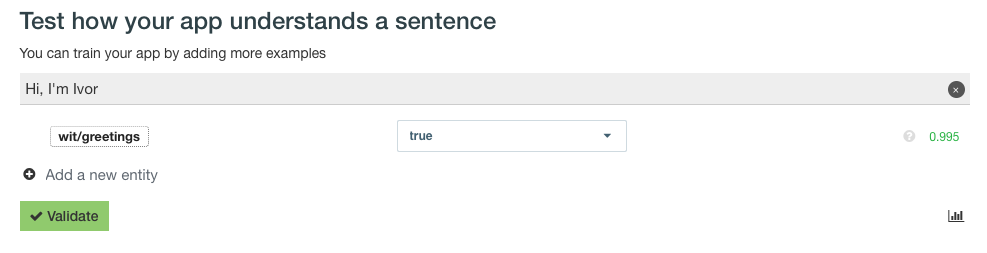
\includegraphics[height=4cm]{img/wit_intents.png}
	\caption{Intent aanmaken Wit.ai}
	\label{fig:intentsWit}
\end{figure}

Wit herkent dit al automatisch als een 'Greeting', hier zie je ook het percentage van 99 percent. Dit percentage is zoals bij LUIS de zekerheid dat Wit denkt dat een intent bij een bepaalde utterance hoort. Indien Wit deze niet herkent of de intent bestaat simpelweg nog niet, kan deze hier aangemaakt en toegevoegd worden. Dit werkt juist op dezelfde manier bij het toevoegen van een entity.

Het weergeven van de al ingevoerde utterances verschilt ook van LUIS. In Wit is er een tabblad 'Samples' waarbij alle utterances worden getoont onder elkaar. Hier kan je de utterances filteren per intent.

\begin{figure}[h!]
	\centering
	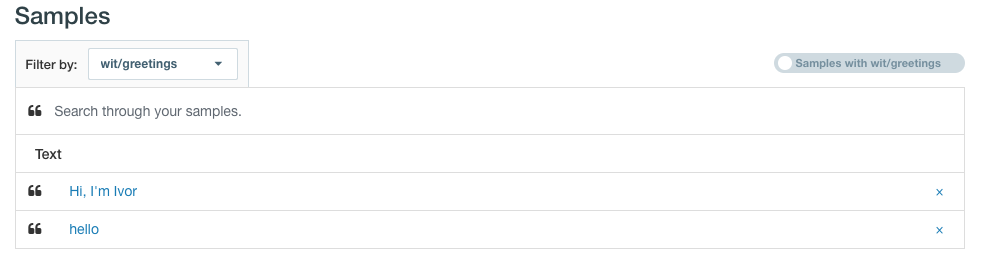
\includegraphics[height=4cm]{img/samples.png}
	\caption{Intent aanmaken Wit.ai}
	\label{fig:samples}
\end{figure}

Ook heeft Wit net zoals LUIS een pagina waar de utterances inkomen van de gebruikers die praten met de bot waarvan Wit niet exact weet bij welke intent deze horen. Hierin suggereert wit ook aan de hand van een percentage bij welke intent hij denkt dat een bepaalde utterance hoort. Deze kun je dan ook nakijken of dit klopt, indien dit niet juist is kan je deze veranderen via de dropdown en deze dan valideren. De gevalideerde utterance wordt daarna toegevoegd aan de lijst van de samples met zijn intent.

Ook bij Wit zouden deze reviews moeten geautomatiseerd worden. Nu de basiswerking van Wit duidelijk is geworden, kan er worden gekeken naar de toegankelijkheid van de API. 

\begin{figure}[h!]
	\centering
	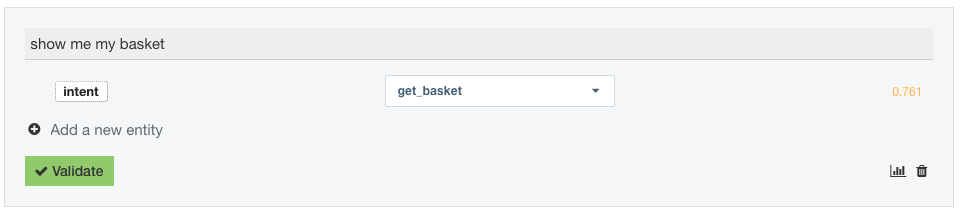
\includegraphics[height=4cm]{img/inbox.png}
	\caption{Intent aanmaken Wit.ai}
	\label{fig:inbox}
\end{figure}

Wit heeft ook wel degelijk een API ter beschikking. De API lijkt zeer sterk op deze van LUIS, er kunnen nieuwe utterances aan worden toegevoegd, samen met nieuwe intent en entities. Ook kunnen hier de utterances worden opgehaald die al gelinkt zijn aan een bepaalde intent. Net zoals bij LUIS zijn de utterances waarvan Wit niet zeker weet bij welke intent ze horen hier niet bij. Deze zullen dus via de webpagina zelf moeten gevalideerd worden en zal niet automatisch kunnen gecontroleerd worden.

\subsection{IBM Watson Assistant}
\label{watson}

Een derde framework voor het bouwen van chatbots is IBM Watson Assistant. Dit framework werkt ook gedeeltelijk op een andere manier dan de vorige onderzochte frameworks. Voor het ontwikkelen van een chatbot in IMB Watson Assistant zijn er drie grote stappen.

De eerste stap is het maken van een 'Skill'. Onder de skill bevindt zich alle logica van de bot, de bot wordt hier getraind. Een skill kan hier vergeleken worden met een App dat je eerst moet maken bij de vorige frameworks. Eerst en vooral dien je een skill aan te maken. Een skill heeft een naam, de taal waarin tegen de bot zal gesproken worden en eventueel een omschrijving. Eénmaal  deze skill is aangemaakt kan je zeer eenvoud intents maken en aan elke intent utterances toevoegen.

\begin{figure}[h!]
	\centering
	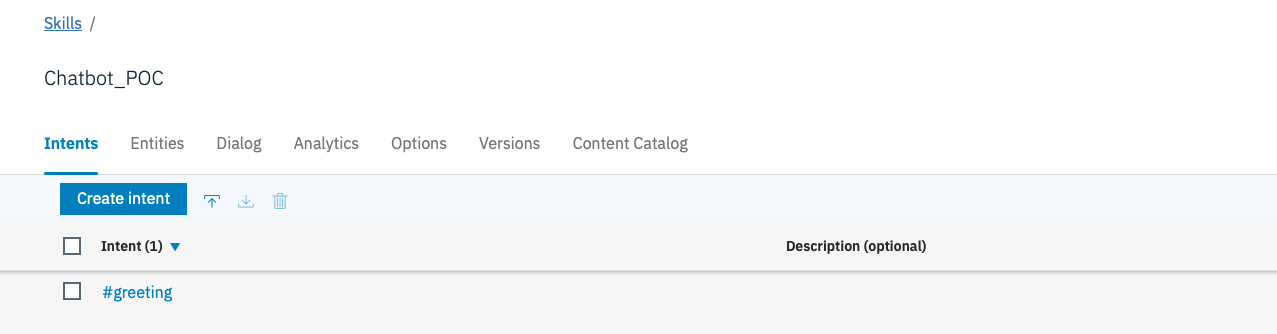
\includegraphics[height=4cm]{img/ibm_intents.png}
	\caption{Intent aanmaken IBM Watson Assistant}
	\label{fig:intentsIbm}
\end{figure}

Na het aanmaken van een bepaalde intent wordt er naar de detailpagina van deze intent genavigeerd. Op deze pagina kan je utterances toevoegen aan deze intent. De werking van dit toevoegen lijkt zeer sterk op die van LUIS. Een entity kan hier ook zeer makkelijk aangeduid worden door de gewenst woorden te selecteren en de juiste entity aan te klikken. Indien de entity nog niet bestaat kan je deze hier even snel direct aanmaken en toewijzen.

\begin{figure}[h!]
	\centering
	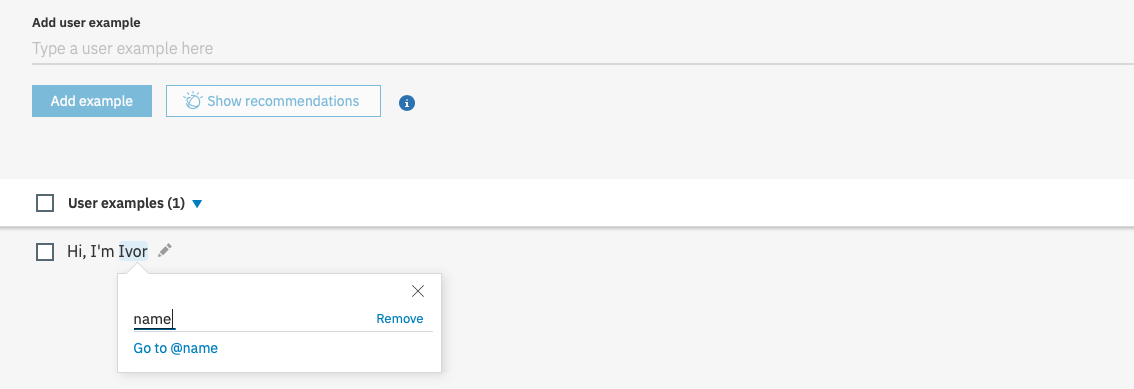
\includegraphics[height=4cm]{img/imb_utterances.png}
	\caption{Utterances toevoegen IBM Watson Assistant}
	\label{fig:utterancesIbm}
\end{figure}

Het trainen van de Skill gaat hier vanzelf. Daarna kan de bot al eens getest worden met de al toegevoegde intents en entiteiten. Als voorbeeld kan er weer worden ingegeven 'Hi, I'm Ivor'. Er kan al direct worden gezien aan welke intent de utterance wordt gelinkt. In vergelijking met LUIS en Wit zijn er hier bij het testen geen percentages. Er is dus niet geweten hoeveel percent de Skill zeker zeker is van een bepaalde intent. Ook kan er direct gezien worden welke entities er worden herkent. Dit wordt getoond in figuur \ref{fig:tryIbm}.

\begin{figure}[h!]
	\centering
	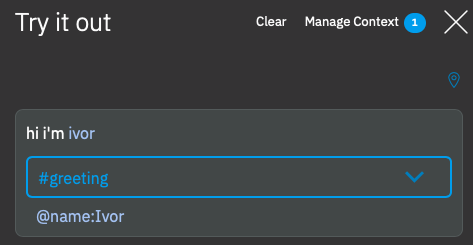
\includegraphics[height=4cm]{img/ibm_try.png}
	\caption{testen van de Skill IBM Watson Assistant}
	\label{fig:tryIbm}
\end{figure}

De tweede stap in dit proces is het deployen van de skill met een assistant. In deze stap wordt de skill aan een assistant gelinkt. Hierin is het eerst nodig om een nieuw assistant te maken. Alleen een naam is vereist, een beschrijving is optioneel. Eénmaal de assistant is gecreeërd, kan er een skill worden aan toegevoegd. Daarna kan je een kanaal kiezen waarop je de bot kan deployen. Hierbij is er ook een preview waarop kan getest worden.

De utterances waarvan de assistant niet zeker is bij welke intent hij hoort worden bijgehouden en kunnen teruggevonden worden onder het tabblad 'Analytics'. Hier kan je doorklikken naar de 'Weak understandings'. Hierin kan je de utterances linken aan de juiste intent. Wat verschillend is met vorige frameworks is dat de assistant geen enkele intent aanbeveeld aan de hand van scores. Hier moet er 100 percent zelf worden nagedacht bij welke intent deze hoort.

\begin{figure}[h!]
	\centering
	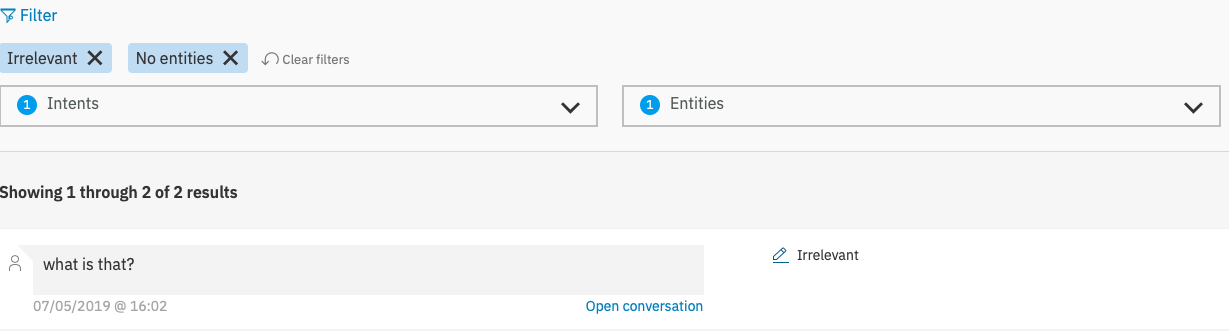
\includegraphics[height=4cm]{img/weak.png}
	\caption{weak understandings IBM Watson Assistant}
	\label{fig:weak}
\end{figure}

IBM Watson Assistant heeft ook een API. Deze API is zeer uitgebreid en bevat zo goed als alle aspecten van de site zelf. Van het creëren van een intent tot het toevoegen van nieuwe utterances en veel meer. In vergelijking met vorige frameworks heeft de assistant van IBM ook een endpoint voor het ophalen van utterances waarvan de assistant niet zeker is. Het enige probleem hier is dat IBM geen scores voorziet bij een utterance dus zal er altijd manuele controle nodig zijn. De ongelinkte utterancers kunnen hier wel opgehaald worden met een eigen applicatie maar de scores ontbreken dus zal er niet automatisch kunnen gecontroleerd worden of deze utterance is gelinkt met de juiste intent.

\subsection{Dialogflow}
\label{dialogflow}

Dialogflow is een chatbot framework gemaakt door google. Net zoals de vorige frameworks heb je hier de mogelijkheid om op een relatief eenvoudige manier een chatbot op te zetten. Hierbij is de eerste stap om een 'Agent' te maken. Dit wordt gedaan door de naam van de Agent, de taal die je tegen de bot zal praten en de tijdzone in te geven.

Een intent aanmaken is hier ook zeer eenvoudig, dit kan door de naam van de intent in te geven. Daarna kunnen er al direct utterances aan toegevoegd worden bij 'Training phrases' zoals er wordt getoont in afbeelding \ref{fig:intentsdialogflow}. De entities kunnen ook toegevoegd worden aan de intent door deze te selecteren en de juiste entity te kiezen. Hierbij zijn er al een aantal ingebouwde entities voorzien. Indien de entity niet in de lijst staat kan er een nieuwe worden aangemaakt in het 'Entities' tabblad, dit kan eenvoudigweg door de naam van de entity in te vullen.

\begin{figure}[h!]
	\centering
	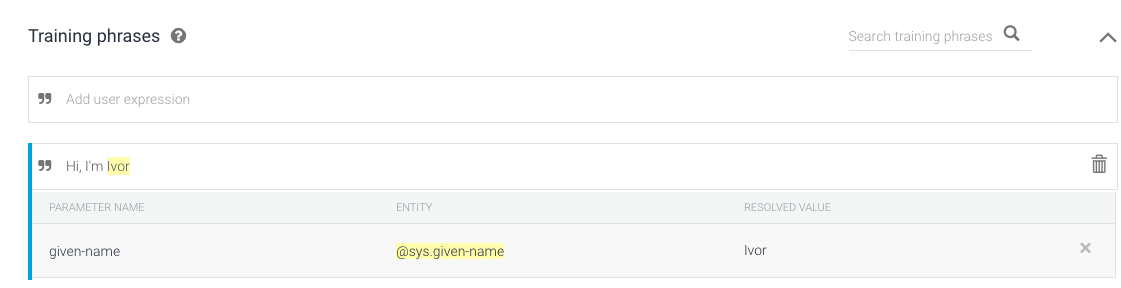
\includegraphics[height=4cm]{img/dialogflow_intents.png}
	\caption{Intent aanmaken Dialogflow}
	\label{fig:intentsdialogflow}
\end{figure}

Deze gemaakte intents met de toepasselijk toegevoegde utterances kunnen al direct getest worden door de console die is voorzien. Er kan al voorbeeld 'Hi, I'm Ivor' gebruikt worden. Hierin kan gezien worden op afbeelding \ref{fig:testdialogflow} dat deze input wordt geanalyseerd door de bot. Deze ziet dat de voorbeeldzin past bij de juiste intent 'Greeting' en dat de waarde 'Ivor' een entity is.

\begin{figure}[h!]
	\centering
	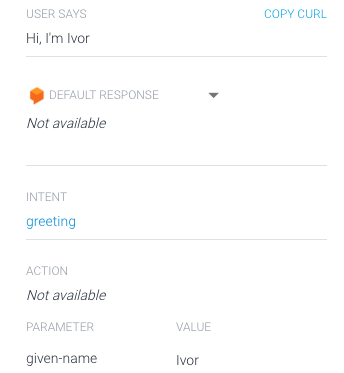
\includegraphics[height=6cm]{img/dia_test.png}
	\caption{Intent aanmaken Dialogflow}
	\label{fig:testdialogflow}
\end{figure}

\subsection{Andere frameworks}
\label{andereFrameworks}



\subsection{Conclusie frameworks}
\label{conclusieFrameworks}



%botframework SDK

%API

%%next chapter POC

%%chapter testen en grafieken en percentages van aantal automatisch

